\section{Episodes and a common end for independent guesses}
\label{episode:section}

A correct clock calculation needs a common clock anchor. A suffix may
propose a different origin or even a different role from the prefix, so
its own local description cannot be assumed to give that anchor. We
therefore define episodes by a rule that can be checked from later
letters, and require a guard comparing every possible outer origin.

Two end searches have different responsibilities. The smaller search
helps define the episode endpoint; the larger search supplies a bounded
clock anchor whenever possible. Their distinction also makes the later
decoder able to evaluate false origins without seeking a new mismatch
past the actual end. Before defining episodes, we place every bounded
inspection for every allowed displacement inside the eventual episode.

\subsection{Two bounded end searches}

Use Lemma~\ref{marker:local} independently of the inner markers, with
integer parameters
\begin{equation}\label{episode:marker-parameters}
 S_\bullet>4(h+w+1),\qquad
 d_\bullet>10BS_\bullet+10(h+w+1),\qquad
 K_\bullet>3d_\bullet^2.
\end{equation}
Call the resulting markers \emph{end markers} and their inspection radius
$r_\bullet\ge K_\bullet$.  For $0\le u<B$ set
\begin{equation}\label{episode:end-widths}
 D_u^0=d_\bullet+uS_\bullet,
 \qquad D_u^1=3d_\bullet+uS_\bullet.
\end{equation}
The center of an end search is $z_\bullet(t)=t+o_\bullet$, where the fixed
offset $o_\bullet$ will be placed below.  At an integer origin $t$, define
$\eta(t)$ and $\zeta(t)$ by the following rule, using $\sigma=0$ and $1$,
respectively: return the leftmost end marker $m_e$ such that
\begin{equation}\label{episode:eligibility}
 |m_e-z_\bullet(t)|\le D_u^\sigma,
 \qquad u=(m_e-z_\bullet(t))\bmod B.
\end{equation}
Return $\bot$ if there is no such marker.  Residues used as indices always
have representatives in $\{0,\ldots,B-1\}$.  These are bounded searches:
the whole inspection is contained in the interval obtained by enlarging
$[z_\bullet(t)-\max_uD_u^\sigma,z_\bullet(t)+\max_uD_u^\sigma]$
by $r_\bullet$ on each side.

The eligible set for $\eta(t)$ is contained in that for $\zeta(t)$.
This does not say that their returned markers coincide: the larger search
may have an earlier eligible marker. The implication we will need also
holds across nearby origins:
\begin{equation}\label{episode:nested-searches}
 |t-t'|\le2h\text{ and }\eta(t')\ne\bot
 \quad\Longrightarrow\quad \zeta(t)\ne\bot.
\end{equation}
Indeed, the marker returned at $t'$ is within
$\max_uD_u^0+2h$ of $z_\bullet(t)$, whereas
\[
 \min_uD_u^1=3d_\bullet>
 d_\bullet+(B-1)S_\bullet+2h=\max_uD_u^0+2h.
\]
It is therefore eligible at $t$ regardless of its new residue index.
This implication is why two search sizes are used.

If $\eta(t)=\bot$, there is no end marker in
$[z_\bullet(t)-d_\bullet,z_\bullet(t)+d_\bullet]$.  The seed
\begin{equation}\label{episode:seed}
 [z_\bullet(t),z_\bullet(t)+K_\bullet)
\end{equation}
then has a period less than $d_\bullet$ by
Lemma~\ref{marker:local}.  Its two-sided continuation with a period less
than $d_\bullet$ is unique: any two such continuations agree on the seed,
whose length exceeds the product of their periods, so
Lemma~\ref{marker:periodic} identifies them.  We shall use this continuation
only when $\eta(t)$ is absent.

\subsection{Margins and the episode rule}

We first identify every bounded window that must remain inside a complete
episode.  This prevents an incorrect origin or endpoint from making a
required check disappear.  Set
\[
 \Delta=(\mathcal H-\mathcal H)\cup(\mathcal P-\mathcal P)\cup\{0\}.
\]
The first difference set contains every displacement of an outer suffix
origin from the true origin at a genuine outer cut, even if the two
factors choose different roles.  The second contains all origin
displacements used to decode an early cut.  Both are fixed finite sets.

For inner data allow every origin displacement in $\Delta$, followed by
every additional integer shift in $[-w_0,w_0]$.  Include all indices
$0\le u<B$, all inner marker inspections, the extended searches through
$H_u+H_{\rm ext}$, the short-period blocks and the finite portions of their
continuations used in Lemma~\ref{schedule:periodic-cuts}, and the finite cut
schedules.  This gives a
bounded integer offset interval $[A_{\rm in},B_{\rm in}]$ relative to $t$.
For example, it may be chosen to contain every enlarged interval
\[
 [o_j+\delta-v-r,
   o_j+\delta+v+H_u+H_{\rm ext}+K+r]
 \quad
 (\delta\in\Delta,\ 0\le v\le w_0),
\]
and every cut offset; enlarge it further if necessary to contain the
$|M|$ periods before the base cuts in
Lemma~\ref{schedule:periodic-cuts}.  All these enlargements are finite and
fixed at this point.

For end data allow every displacement in $\Delta$ and every additional
integer shift in $[-w,w]$.  Include both end-search inspection windows,
every seed, every possible bounded marker return, and the right endpoint
of every seed.  Collect them in a bounded integer interval
$[A_{\rm end},B_{\rm end}]$ relative to $z_\bullet(t)$. For clarity, an
interval containing the following sets, over all $\delta\in\Delta$ and
$|v|\le w$, is sufficient:
\[
 [\delta+v-\max_uD_u^1-r_\bullet,
   \delta+v+\max(\max_uD_u^1+r_\bullet,K_\bullet)].
\]
In particular these intervals cover full sweeps of the allowed shifts,
not merely the finitely many nominal origins.  Neither interval depends
on the still unchosen $L,o_\bullet,L_{\rm tail}$.

Choose positive integers $L,o_\bullet,L_{\rm tail}$ in this order so that
\begin{equation}\label{schedule:margin-inequalities}
 \begin{split}
 L+A_{\rm in}&>\beta_{g'},\\
 o_\bullet+A_{\rm end}&>B_{\rm in},\\
 L_{\rm tail}&>\max\{1,\max_uD_u^0+B_{\rm end}\}.
 \end{split}
\end{equation}
Now fix $t=s+L$ for a word beginning at $s$.  Define its \emph{end anchor}
$q_0$ as follows.  If $\eta(t)$ is present, put $q_0=\eta(t)$.  Otherwise
use the unique periodic continuation of the seed in
\eqref{episode:seed}, and let $q_0$ be the first letter position at or
beyond the seed's right endpoint where the word differs from that
continuation.  If that mismatch has not yet occurred in a finite word,
the rule supplies no complete episode in that word.  When $q_0$ exists,
the required endpoint is
\begin{equation}\label{episode:endpoint}
 b=q_0+L_{\rm tail}.
\end{equation}
All bounded end inspections and seed data required by the rule must be
available, as must the letters through $b-1$.  A word is a \emph{complete
episode} if its own endpoint is exactly this $b$.  Let $E$ be the language
of such words, with their beginning normalized to $s=0$.  For each complete
episode define the \emph{clock anchor}
\begin{equation}\label{episode:clock-anchor}
 q=\begin{cases}
     \zeta(t),&\zeta(t)\ne\bot,\\
     q_0,&\zeta(t)=\bot.
    \end{cases}
\end{equation}
These two anchors have different roles and may coincide. The endpoint is always
$q_0+L_{\rm tail}$. The clock instead uses $q$, which is a bounded
marker return whenever $\zeta$ is present. For example, $\eta$ may be
absent and $\zeta$ present; then the endpoint can occur arbitrarily late
at a first mismatch while its clock anchor remains bounded. No later
argument identifies $q$ with $q_0$ in this case.

\begin{lemma}[Internal data under all prescribed hypotheses]
\label{schedule:margins}
The choices above place every bounded inner window after $b'_{g'}$, every
bounded end window after every outer cut, and all these windows strictly
inside every complete episode.  These assertions hold simultaneously for
all the origin displacements and additional shifts just specified.
\end{lemma}

\begin{proof}
The first two claims are the first two inequalities in
\eqref{schedule:margin-inequalities}.  In either branch of the episode
rule,
\[
 q_0\ge z_\bullet(t)-\max_uD_u^0.
\]
Consequently the last inequality gives
\[
 b=q_0+L_{\rm tail}>z_\bullet(t)+B_{\rm end},
\]
past every bounded end window, and hence past all the earlier windows.
The first inequality also puts all these windows after the beginning
$s=b'_0$.  The same bounds apply on any continuation of the word.
\end{proof}

Figure~\ref{schedule:schematic} summarizes the order just established.  The
large gaps also accommodate the false origins; they are not chosen anew
after a suffix has made its guesses.
\begin{figure}[htbp]
\centering
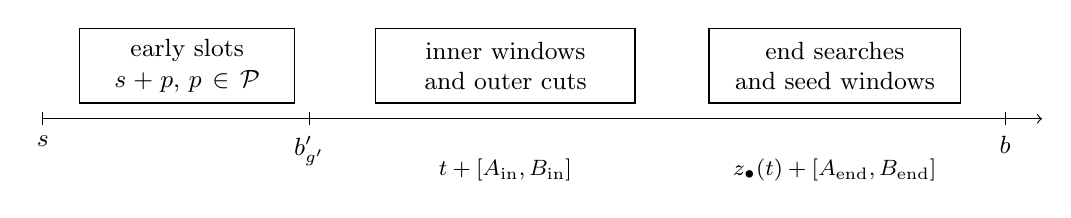
\begin{tikzpicture}[x=.94cm,y=1cm,font=\small]
 \draw[->] (0,0)--(13.5,0);
 \draw (0,-.08)--(0,.08) node[below=5pt] {$s$};
 \draw (13,-.08)--(13,.08) node[below=5pt] {$b$};
 \draw (.5,.2) rectangle (3.4,1.15);
 \node[text width=2.5cm,align=center] at (1.95,.675)
   {early slots\\$s+p$, $p\in\mathcal P$};
 \draw (4.5,.2) rectangle (8,1.15);
 \node[text width=3cm,align=center] at (6.25,.675)
   {inner windows\\and outer cuts};
 \draw (9,.2) rectangle (12.4,1.15);
 \node[text width=2.9cm,align=center] at (10.7,.675)
   {end searches\\and seed windows};
 \draw (3.6,-.08)--(3.6,.08) node[below=5pt] {$b'_{g'}$};
 \node[font=\footnotesize,align=center] at (6.25,-.65)
   {$t+[A_{\rm in},B_{\rm in}]$};
 \node[font=\footnotesize,align=center] at (10.7,-.65)
   {$z_\bullet(t)+[A_{\rm end},B_{\rm end}]$};
\end{tikzpicture}
\caption{The order of bounded data in a complete episode, schematically
and not to scale.  Both window intervals include every prescribed shifted
hypothesis.  The end anchor may be a bounded marker return or a later
first mismatch; in either case the fixed tail puts $b$ beyond all bounded
end data.}\label{schedule:schematic}
\end{figure}

\FloatBarrier

For every prefix or suffix test below, the letters needed for a check
must be present in that test's own argument and on its own reading side.
An unavailable inspection or an invalid required product interval causes
rejection; it never removes an origin from a universal check.  The
unbounded portions of the episode rule are continuation tests up to a
proposed end.  They do not require moving an unbounded inspection window
before a cut.  Lemma~\ref{schedule:inner-cuts} supplies the more precise
division of inner data between the two sides of an outer cut.

\begin{lemma}\label{episode:prefix-code}
The language $E$ is a prefix code of nonempty words.
\end{lemma}

\begin{proof}
Suppose that a complete episode is read from its beginning in a longer
word.  By Lemma~\ref{schedule:margins}, every bounded search and seed
inspection lies inside the episode, so locality gives exactly the same
search values on the longer word.  If $\eta$ is present, it gives the same
$q_0$.  If it is absent, the seed gives the same continuation, and the
already encountered first mismatch remains the first mismatch.  Thus
$q_0$, and hence $b$, cannot change.  No complete episode can be a proper
prefix of another.  Positivity follows from the strict ordering in
Lemma~\ref{schedule:margins} and from $L_{\rm tail}>1$.
\end{proof}

All these definitions commute with translation of positions.  A standalone
prefix reads from its beginning $s$ to its end $k$.  A standalone suffix
begins at $k$; an origin specified as an offset from $k$ need not itself
carry a visible letter in that suffix.  Applying the end rule at such an
origin requires the end searches and seed in the suffix and its prescribed
exact endpoint.  It does not ask the suffix to validate omitted prefix
letters.

\subsection{A guard that forces the true end}

At a proposed outer cut $k$, let the suffix test all origins
\begin{equation}\label{episode:outer-origins}
 \mathcal O_k=\{k-a:a\in\mathcal H\}.
\end{equation}
Choose once and for all a reference offset in $\mathcal H$.  The
\emph{common end guard} requires both $\eta$ and $\zeta$ to be constant
across $\mathcal O_k$, with equality of absolute positions or of the value
$\bot$.  Require all the associated bounded inspections and seed blocks.
The suffix must end exactly where the episode rule at the reference
origin prescribes, and uses the clock anchor calculated there by
\eqref{episode:clock-anchor}.

\begin{lemma}[Shared end and clock anchor]\label{episode:shared-end}
Let a word in $E^*$ have first episode beginning at $s$, sampling origin
$t=s+L$, endpoint $b$, and clock anchor $q$.  Let $k=t+a$ be any genuine
outer cut, with $a\in\mathcal H$.  If a suffix starting at $k$ satisfies
the common end guard, then its consumed endpoint is exactly $b$ and the
clock anchor it uses is exactly $q$.

Conversely, the actual suffix of that episode from $k$ to $b$ satisfies
the guard whenever both end searches at $t$ are unchanged under every
shift divisible by $B$ with absolute value at most $w$.
\end{lemma}

\begin{proof}
Because $k=t+a$ for an actual offset $a\in\mathcal H$, the set
$\mathcal O_k$ contains $t$. All its other origins differ from $t$ by
$\mathcal H-\mathcal H$. Lemma~\ref{schedule:margins} puts their
bounded end data inside the first episode and after $k$. A proposed
suffix must supply every one of these windows. If it is too short it
rejects; otherwise it reads the genuine letters in those windows, even
if its endpoint proposal is false.

Suppose first that the common value of $\eta$ is a marker. Since $t$
is among the origins, this value is the episode's own $q_0$, and the
reference end test demands $q_0+L_{\rm tail}=b$.

In the remaining case all smaller searches are absent. Let $t_*$ be the
reference origin. Its seed and the true seed start less than
$w<d_\bullet$ apart and overlap in at least
$K_\bullet-w>d_\bullet^2$ letters. Their short-period continuations are
therefore identical by Lemma~\ref{marker:periodic}. The word agrees
with that continuation on both seeds and hence on their union. If one
seed ends earlier, there is still agreement through the end of the later
seed. Consequently the first mismatch after either seed is one and the
same position. An alleged earlier mismatch contradicts that agreement
or the true first-mismatch property. An alleged later one would pass the
true first mismatch. Thus the reference exact-end test again forces $b$.
The common value of $\zeta$ now also forces $q$: it is the true bounded
return when present, and the common $q_0$ otherwise.

Conversely, every displacement from $t$ to a member of $\mathcal O_k$
is divisible by $B$ and has magnitude less than $w$. The assumed
stability makes each search constant on this set. All windows are
available in the actual suffix by the margin lemma. A common marker
return fixes the true end immediately; in the absent case the seed
argument above fixes the common first mismatch. Hence the reference
end test succeeds and supplies the true clock anchor.
\end{proof}

We can now use the clock with genuinely independent prefix and suffix
metadata.  Even if their proposed roles differ, the guard ensures that
the two clock arguments add to the true total $\varphi(q-t)$.
